%%%%%%%%%%%%%%%%%%%%%%%%%%%%%%%%%%%%%%%%%%%%%%%%%%%%%%%%%%%%%%%%%%%%%%%%%%%%%%%
% Fractio of gluon splitting in data
%%%%%%%%%%%%%%%%%%%%%%%%%%%%%%%%%%%%%%%%%%%%%%%%%%%%%%%%%%%%%%%%%%%%%%%%%%%%%%%
%
\chapter{Fraction of double $b$-hadron jets in QCD $b$-production}\label{ch:gbbfraction}


In this chapter we apply the newly developed $g->b\bar{b}$ tagging tool to measure the fraction of merged $b$-jets in QCD $b$-jet production. The fractions are determined both for an inclusive $b$-jet sample with $|\eta|<2.1$, and for exclusive samples enriched in single or in merged $b$-jet.
The measured fractions are in excellent agreement within the experimental uncertainties with the theoretical prediction from a parton shower Monte Carlo simulation of hadronic collisions.
The chapter is organized as follows. Section~\ref{sec:FitIntro} introduces the concept of template fitting. Section~\ref{sec:LLFits} describes the statistical method used to perform the template fits.
BLABLABLABLABLA

%------------------------------------------------------------------------
\section{Introduction}
%------------------------------------------------------------------------

The $g\rigtharrow b\bar{b}$ tagger developed and described in the previous chapters produces for every $b$-tagged jet a number between 0 and 1, the double $b$-hadron likelihood (LL). The closer this number if to 1 (0), the more likely the $b$-tagged jet is single (merged). When used as a tagger, a working point (Wp) is chosen so that if LL$\geq$Wp the jet is flagged as single. The value of the Wp is chosen as a compromise between good efficiency (the lower the Wp, the higher the probability that an actual single $b$-jet will not be missed by the tagger), and rejection power (the higher the Wp the higher the probability that a non-single $b$-jet will not be incorrectly flagged as single). Depending on the necessities of the particular analysis, an appropriate Wp is to be chosen form the plot in Figure~\ref{fig:performanceinbins}, and in particular the performance results presented in Chapter~\ref{ch:mva} correspond to 50\% and 60\% efficiency working points, a reasonable choice.

However, the values of LL in a given sample offer more information than just a jet-by-jet tagger: the distribution of LL allows to measure the composition of the particular sample. In effect, a $b$-tagged jet has a certain probability to actually originate from the hadronization of a:

\begin{description}
\item[$\bm b$]: $b$-quark
\item[$\bm bb$]: gluon splitting into a $b\bar{b}$ pair
\item[$\bm c$]: $c$-quark
\item[$\bm cc$]: gluon splitting into a $c\bar{c}$ pair
\item[$\bm \ell$]: light parton ($u$, $d$, $s$ quarks, or a $g$ not splitting into heavy flavor pair).
\end{description}

\emph{The expected distribution of LL is different for each of the five cases. This is illustrated in Figure~\ref{templates}, which plots LL for each hypothesis for jets in two $\pt$ ranges ($40<\pt\leq60$~GeV and $200<\pt\leq270$~GeV). These distributions are henceforth called ``templates''}. One can determine the composition of a given sample by measuring the values of LL of the $b$-tagged jets and estimating the fractions needed from each of the templates to accurately describe the experimental LL distribution. This process is known as ``template fitting''.

\emph{The shape of the templates in Figure~\ref{templates} can be intuitively understood. The $b$ and $bb$ templates behave as expected, respectively peaking at high and low values of LL. The $c$ and $cc$ templates resemble their $b$ counterparts. This was to be expected, given that a $c$-quark fragments mainly into into $D$-mesons which have a measurable $c\tau$ of \~300$\mu$m, although shorter than the  $c\tau$ of \~500$\mu$m corresponding to the $B$-mesons produced in $b$-quark fragmentation. Single and merged $c$-jets are thus the main background to $b$- and $bb$-jets. The template of light jets, on the contrary, do not contain large decay-length secondary vertices, and its distribution is driven by..}



%------------------------------------------------------------------------
\section{Unbinned maximum likelihood fits}\label{sec:LLFits}
%------------------------------------------------------------------------

The analysis of experimental data often involves the estimation of the composition of a sample, based on Monte Carlo description of the various sources.We measure a number of observables $x_i$ and we want to determine one or more parameters $p_i$ from the data, such as the number of signal and background events. The distribution  of the observables is described by a probability density function (PDF), which is a function of %both the observables and 
the parameters, $F(\vec{x},\vec{p})$.  We choose the PDF based on some hypothesis about what function would match the data, and vary the parameters in order to make the PDF match the distribution of the observables as well as possible. 


In the case of data binned into a histogram, one approach is to use a least-squares fitting technique to estimate the parameters. They are adjusted to minimize
%
\begin{equation}
\chi^2 = \sum_i \frac{(d_i - f_i)^2}{d_i}
 \label{eq:chi2}
\end{equation}
%
where $d_i$ is the number of events in the real data that fall into bin $i$, and $f_i$ is the predicted number of events in bin $i$, defined by
%
\begin{equation}
f_i = N_D\sum^m_{j=1} p_j \cdot a_{ji}/N_j
\end{equation}
%
with $p_j$, the proportions of the different $m$ sources; $a_{ij}$, the number of Monte Carlo events from source $j$ in bin $i$, with $i=1,2,...,n$; $N_D$, the total number of events in the data sample; and $N_j$, the total number in the MC sample for source $j$.

This $\chi^2$ assumes that the distribution for $d_i$ is Gaussian and that $a_{ij}$ has no uncertainty; it is of course Poisson, but the Gaussian $N(\mu = d_i,\sigma = \sqrt{d_i})$ is a good approximation to the Poisson for large numbers. Unfortunately it often happens that many of the $d_i$ are small, making the $\chi^2$ value given in Equation~\ref{eq:chi2} inappropiate to describe the problem.  Instead one can go back to the original Poisson distribution, and write down the probability for observing a particular $d_i$ as
%
\begin{equation}
e^{-f_i} \frac{f_i^{d_i}}{d_i!} 
\end{equation}
%
and the estimates of the proportions $p_j$ are found by maximizing the total likelihood, 
%
\begin{equation}
\mathcal{L} = \prod^n_{i=1} e^{-f_i} \frac{f_i^{d_i}}{d_i!}.
\end{equation}
%
This accounts correctly for the small numbers of data events in the bins.  It is often referred to as a ``binned maximum likelihood'' fit. Actually this formalism does not account for fluctuations in the $a_{ji}$ due to finite Monte Carlo samples. A similar methodology that correctly describes this scenario exists, see Ref.~\cite{Barlow1993219}. The effects of finite MC data size can be considered small for MC samples ten times larger than the data sample. 


The binned maximum likelihood fits is a technique in general use. Unfortunately  this method does not behave well in problems where it is necessary to apply weights to the Monte Carlo, such as in our composite dijet sample. We will use instead a different technique for fitting, an ``unbinned maximum likelihood fit'', which does support weighted datasets. %But use with care. Error analysis in ML fits to weighted unbinned data can be complicated...
%Binned or unbinned MF fit. %Roofit presentation page 112
%In most RooFit applications it doesn't matter. Internally binned data is represented the same way as unbinned data, a ROOT TTree with the bin coordinates.

The likelihood to be maximized in an unbinned dataset of events $\{x_k\}^N_{k=1}$ is
%
\begin{equation}
\mathcal{L}(\vec{x};\vec{p}) =\prod^N_{k=1} F(x_k;\vec{p})
\end{equation}
%
which, can be rewritten in terms of the probability of observing an event from source $j$ in the sample,
%
\begin{equation}
\mathcal{L} =  \prod^N_{k=1} \sum^m_{j=1} n_j  \mathcal{P}_j(x_k)
\end{equation}
%
where $\mathcal{P}_j$ are the PDFs that represent the total probability for each of the $m$ hypothesis, $p_j=n_j$ are the parameters representing the number of events for the $j^{th}$ hypothesis, and $N$ is the total number of input data points.

%\subsubsection{Extended maximum likelihood fits}

%Maximum likelihood information only parametrizes the shape of a distribution; that is, one can determine fraction of signal events from MC fits but no number of signal events. The extended version of the maximum likelihood approach adds an extra term allowing the estimation of %the absolute number of signal/background events. 
%a parameter that represents the number of events in the sample, $N_{exp}$.
%The extra term describes the probability of observing the actual number of events, $N_{obs}$, given this parameter. This probability is described by the Poisson distribution
%%
%\begin{equation}
%P(N_{obs},N_{exp}) \sim  N_{exp}^{N_{obs}} \cdot e^{-N_{exp}},
%\end{equation}
%%
%and we refer to the likelihood including this factor as the ``extended likelihood''
%%
%\begin{equation}
%\tilde{\mathcal{L}}(\vec{x},N_{obs};\vec{p},N_{exp}) \equiv P(N_{obs},N_{exp}) \cdot \mathcal{L}(\vec{x};\vec{p})
%\end{equation}
%%
%The fit then finds the values of $n_j$, the number of events for each hypothesis $j$. 


The fits were performed in this thesis by means of the RooFit Toolkit for data modelling~\cite{RooFit}. Performing a fit consists of minimizing the negative log-likelihood of a PDF calculated over the data set % (for simplicity we drop for a moment the extra term)
%
\begin{equation}
-\log \mathcal{L} (\vec{p}) = \sum_k F(\vec{x}_k;\vec{p})
\end{equation}
%
with respect to the model's parameters.  The RooFitTools package uses the MINUIT\cite{MINUIT} algorithms to find the minimum of this function and estimate the errors in each parameter.  %fitTo() method returns an interger status code which is non-zero if the fit fails to converge normally.
%In order to assess the goodness of a fit one can compare the minimum value of the negative log-likelihood function with the expected distribution of values for samples generated according to the fit model (using the Monte Carlo study methods).
To increse the chances of proper convergence, it is important to provide reasonable initial estimates for the parameters to be fitted.


%\subsubsection{Model}

Most realistic data description models are sum of multiple components. Mathematically, the sum of two probability density functions is  also a normalized probability density function as  long as the coefficients add up to 1, % (or to the total number of events for an extended maximum likelihood fit),
%
\begin{equation}
M(x) = f_{sig} \cdot S(x) + (1-f_{sig}) \cdot B(x),
\end{equation}
%
or generically for N components:
%
\begin{equation}
S(x) = c_0 \cdot F_0(x) + c_1 \cdot F_1(x)+...+c_{n-1}F_{n-1}(x)+ (1-\sum^{n-1}_{i=1}c_i) F_n(x)
\end{equation}
%
If the sum of these coefficients becomes larger than one, the remainder coefficient will be assigned a negative fraction. As long as the summed p.d.f is greater than zero everywhere, this is not ill-defined. %but may pose some problems in the interpretation



%For the extended fit (for simplicity we take the example of signal and backgrond PDFs), 
%%
%\begin{equation}
%N_{sig} = f_{sig} \cdot N_{exp}
%\end{equation}
%%
%\begin{equation}
%N_{bkg} = (1-f_{sig}) \cdot N_{exp}
%\end{equation}
%%
%so that the extended ML procedure estimates the number of singal and background events rather than a signal fraction and a total number of events.
%The uncertainties in the yields reported by the fit will include the statistical (      )                  N                    uncertainty.

%Estimated Distance to Minimum should be small O(10-6)



%------------------------------------------------------------------------
\section{Fitting MC templates to data}\label{sec:FitsResults}
%------------------------------------------------------------------------



Likelihood Monte Carlo templates were derived from the simulated dijet sample described in Section~\ref{sec:analysis}, from all jets passing the selection criteria defined in Section~\ref{sec:EventSelection}. Templates of likelihood were constructed for $b$, $c$, $b\bar{b}$, $c\bar{c}$ and light flavoured MV1 tagged jets separately, and these were fitted to the likelihood distribution in data in order to obtain the fractions of single $b$, merged $b$, single $c$, merged $c$ and light jets in the data sample. Merged $c$-jets (single $c$-jets) are defined as those jets matching exactly two (only one) ``$D$'' hadrons, the products of the fragmentation of $c$-quarks. A jet is classified as light when it has no $B$ nor $D$ hadrons within a cone of 0.4 around its axis.

The likelihood template fits are performed using the unbinned maximum likelihood technique, in its extended version (see Section~\ref{sec:LLFits}). A separated fit is carried out for each $\pt$ bin. Different combinations of templates (``models'' in the following) were used to fit the likelihood distribution in data. The first implemented model uses all five templates,
%
\begin{equation}
F(x) = n_s \cdot S(x) + n_m \cdot M(x) + n_l \cdot L(x) + n_{sc} \cdot S_c(x) + n_{mc} \cdot M_c(x)
\end{equation}
%
with $S(x)$, $M(x)$, $L(x)$, $S_c(x)$ and $M_c(x)$ the likelihood PDFs for the different hypothesis; and $n_s$, $n_m$, $n_l$, $n_{sc}$ and $n_{mc}$ the free parameters representing the number of expected events for all components: single $b$, merged $b$, light, single $c$ and merged $c$-jets, respectively.  %The initial estimates for the parameters were obtained from the {\sc Pythia} Monte Carlo sample. 
\emph{The fractions derived in {\sc Pythia}  as a function of the jet $\pt$ are shown in Fig.~\ref{fig:truefractions}.}


\begin{figure}[tp]
\centering
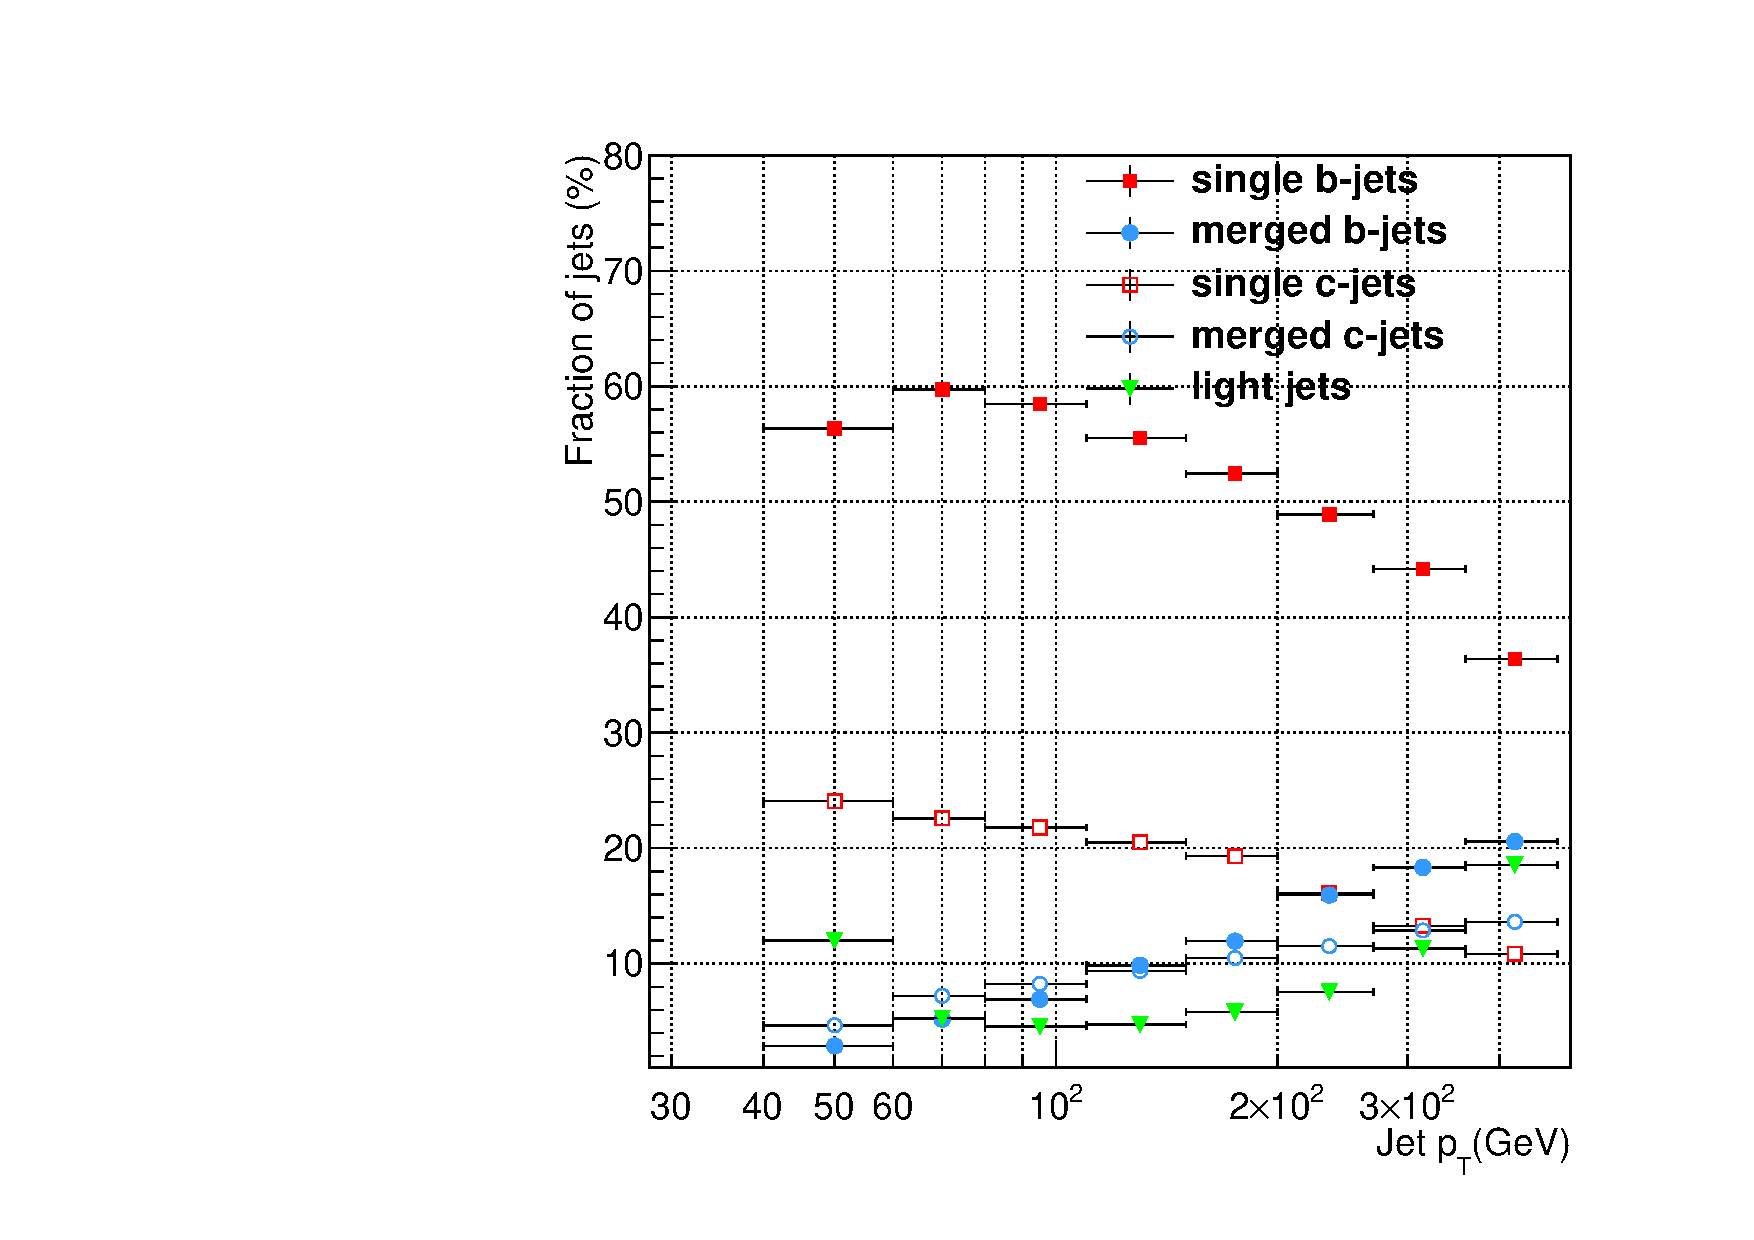
\includegraphics[width=0.70\textwidth]{TrueFractions_NominalPythia.pdf}
%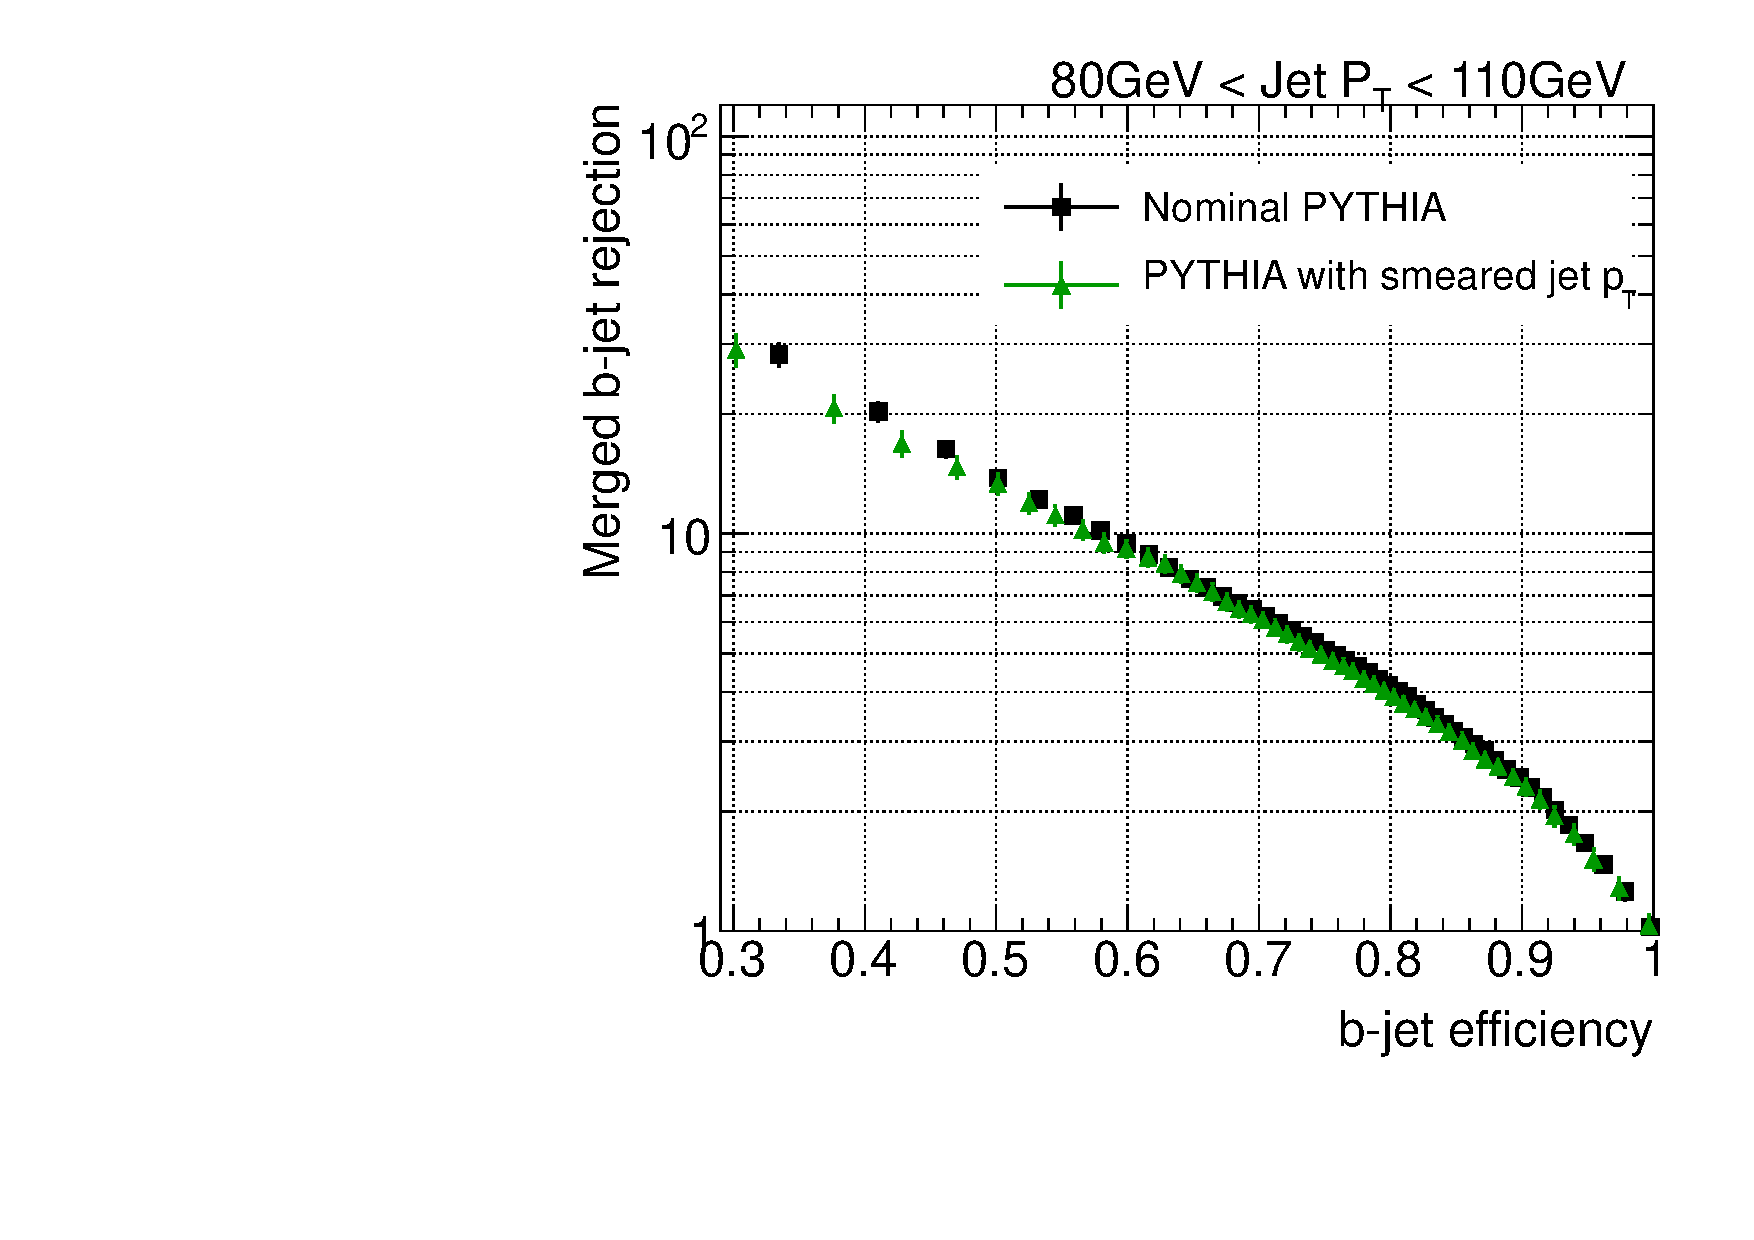
\includegraphics[width=0.49\textwidth]{FIGS/systematics/LlhoodKDE_ISO_SmearedJetPt_FIXEDBUGTest_rejvseff080.pdf}
\caption{Theoretical predictions of the fractions of $b$-, $b\bar{b}$-, $c$-, $c\bar{c}$, and light jets in $b$-tagged {\sc Pythia} QCD sample.}
\label{fig:truefractions}
\end{figure}


The sensitivity of the fit result to fixing the ratio of the single $c$ (merged $c$) fraction, for each $\pt$ bin, and the single $b$ (merged $b$)  one to the value extracted from the simulation was investigated by carrying out separate fits with a model with three free parameters only. This was motivated by the fact that templates for single $c$- (merged $c$-)  and single $b$-jets (merged $b$-jets) look very similar leading to inestabilities in the fitted $b$- and $c$-flavour fractions, caused by the high correlations between these components. 


The results of the template fits to the likelihood distribution in data, using the three-parameter model, are shown in table~\ref{tb:fitfractions}. Examples of this set of fits are displayed in Figures~\ref{fig:fittemplates1} and~\ref{fig:fittemplates2}.


\begin{table}[!hbt] %[h]
\renewcommand{\arraystretch}{1.2}
\centering
\begin{tabular}{ | c || c | c || c | c || c | c ||}
  \hline
  Jet $\pt$ & \multicolumn{2}{c||}{single $b$-jet} & \multicolumn{2}{c||}{merged $b$-jet} & \multicolumn{2}{c||}{~light jet~}\\ \cline{2-7}
    (GeV ) & ~~~$n_s$~~~~ & stat.err. & ~~~$n_m$~~~~ & stat.err.& ~~~$n_l$~~~~ & stat.err.\\ \hline
   40 - 60 &  62\% &  3\%  &  ~~3\%  &  ~~1\% &  ~4\%  &  4\%   \\ 
   60 - 80 &  62\% &  1\%  &  5.2\%  &  0.4\% &  ~2\%  &  2\%   \\ 
   80 - 110&  57\% &  1\%  &  8.5\%  &  0.4\% &  ~3\%  &  2\%   \\ 
  110 - 150&  55\% &  2\%  &  ~13\%  &  ~~1\% &  ~1\%  &  4\%   \\ 
  150 - 200&  53\% &  3\%  &  ~15\%  &  ~~1\% &  ~0\%  &  4\%   \\ 
  200 - 270&  53\% &  5\%  &  ~17\%  &  ~~1\% &  -1\%  &  7\%   \\ 
  270 - 360&  48\% &  3\%  &  ~19\%  &  ~~1\% &  ~4\%  &  4\%   \\ 
  360 - 480&  39\% &  5\%  &  ~21\%  &  ~~1\% &  15\%  &  6\%   \\ \hline
\end{tabular}
\caption{Measured fractions of single, merged and light $b$-tagged jets in experimental data from 2011 run.}
\label{tb:fitfractions}
\end{table}


\begin{figure}[tp]
\centering
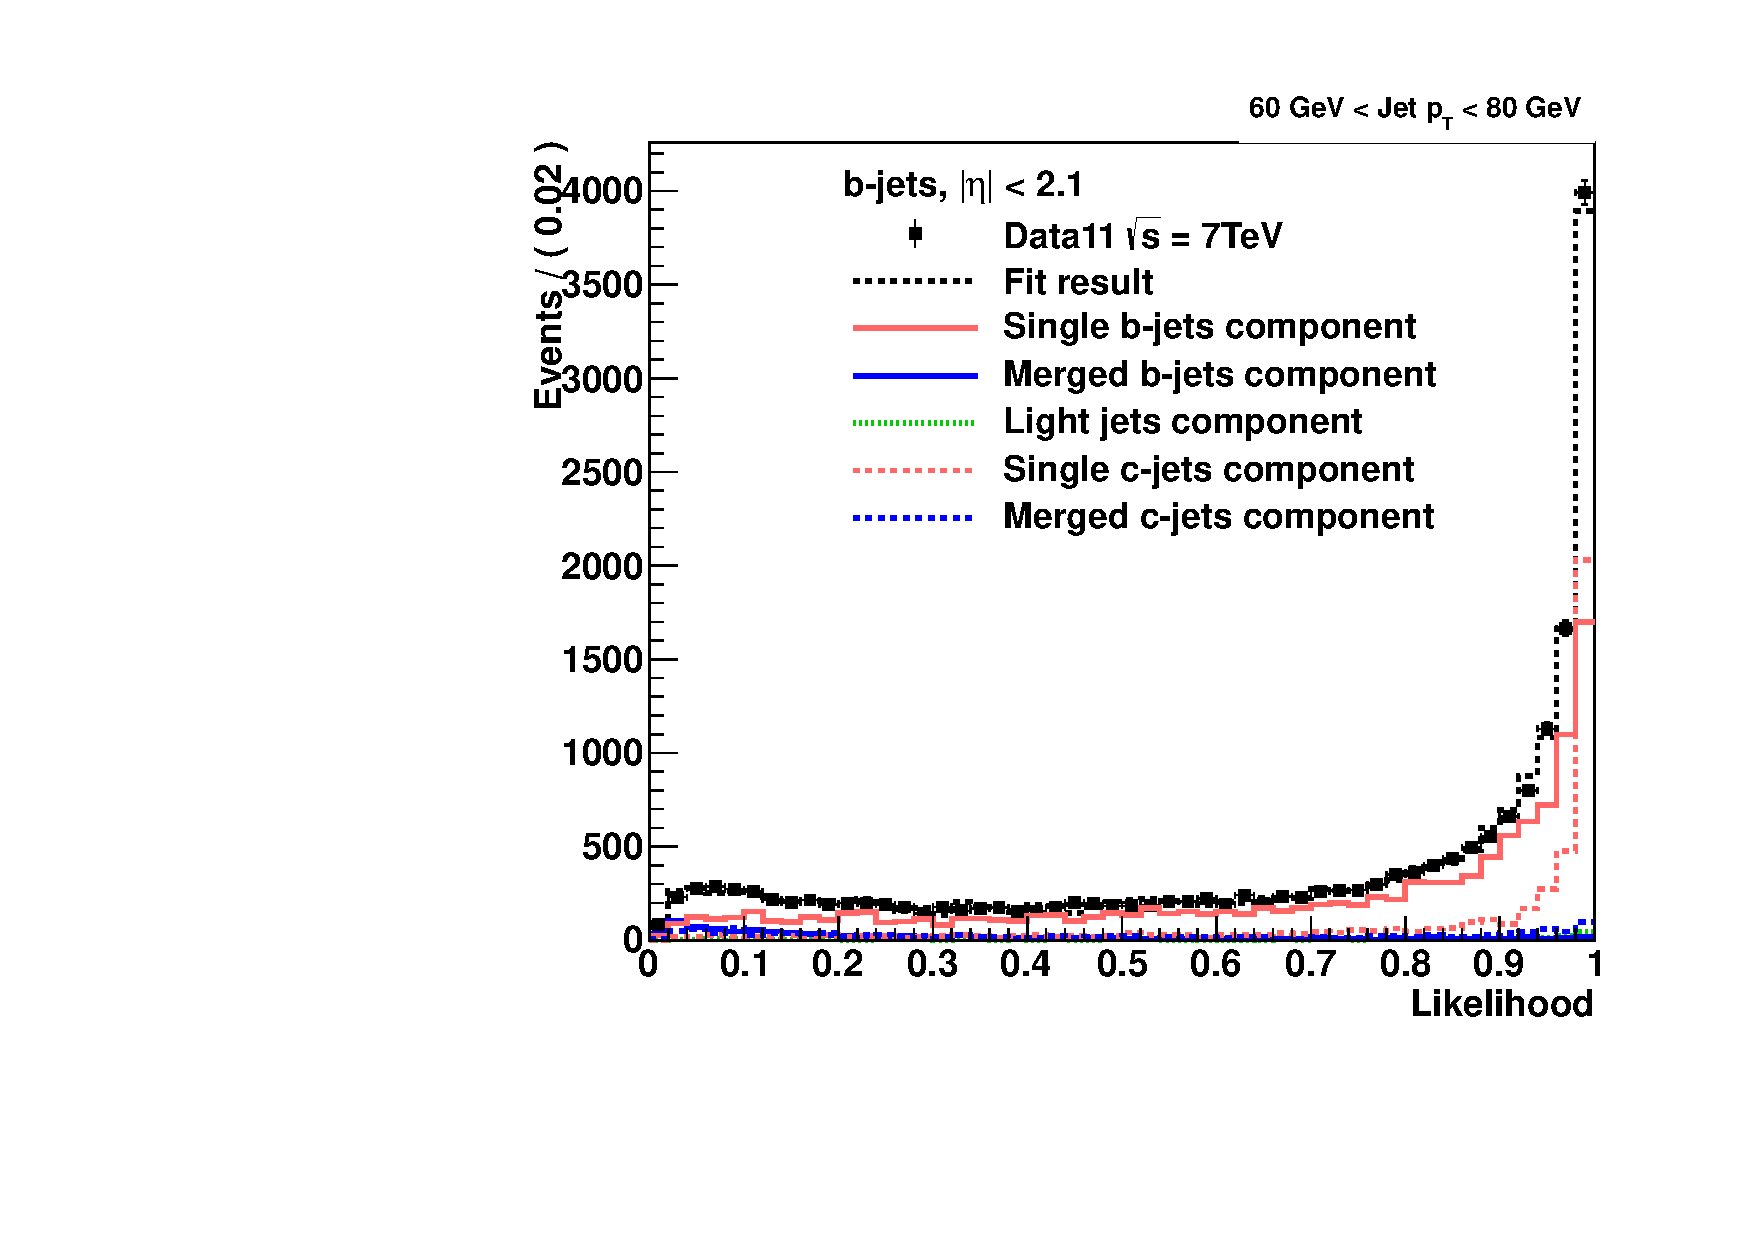
\includegraphics[width=0.7\textwidth]{FIGS/Fits/LikelihoodFit_3param_ETAFull_Bin1.pdf}
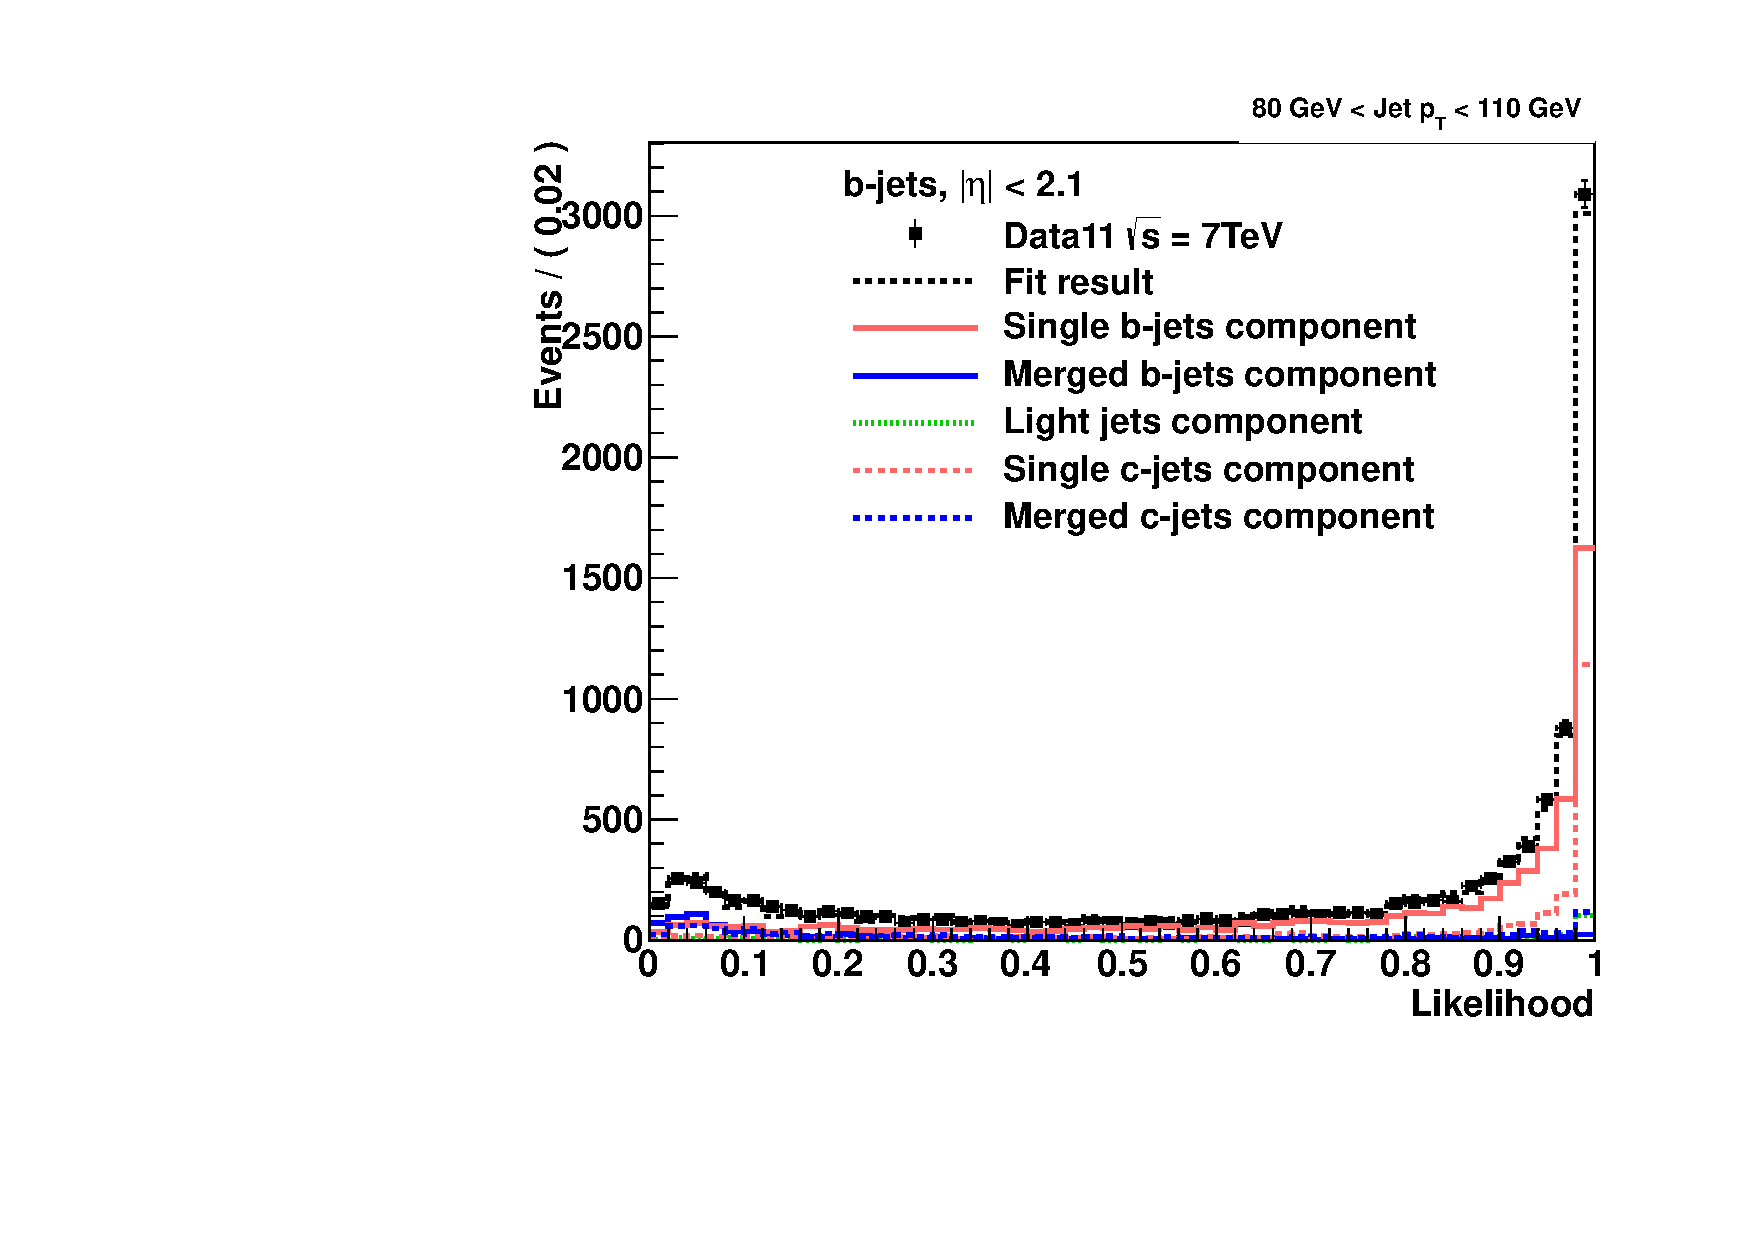
\includegraphics[width=0.7\textwidth]{FIGS/Fits/LikelihoodFit_3param_ETAFull_Bin2.pdf}
\caption{The results of template fits to the likelihood distribution in data. The fits shown here were performed on jets with $\pt$ between  60~GeV and 80~GeV, and 80~GeV and 110~GeV, using five templates of $b$-, $b\bar{b}$-, $c$-, $c\bar{c}$, and light jets.  The ratio of the $c$- to $b$-flavour fractions was fixed to the values observed in the simulation.  Uncertainties shown are for data statistics only.  }
\label{fig:fittemplates1}
\end{figure}



\begin{figure}[tp]
\centering
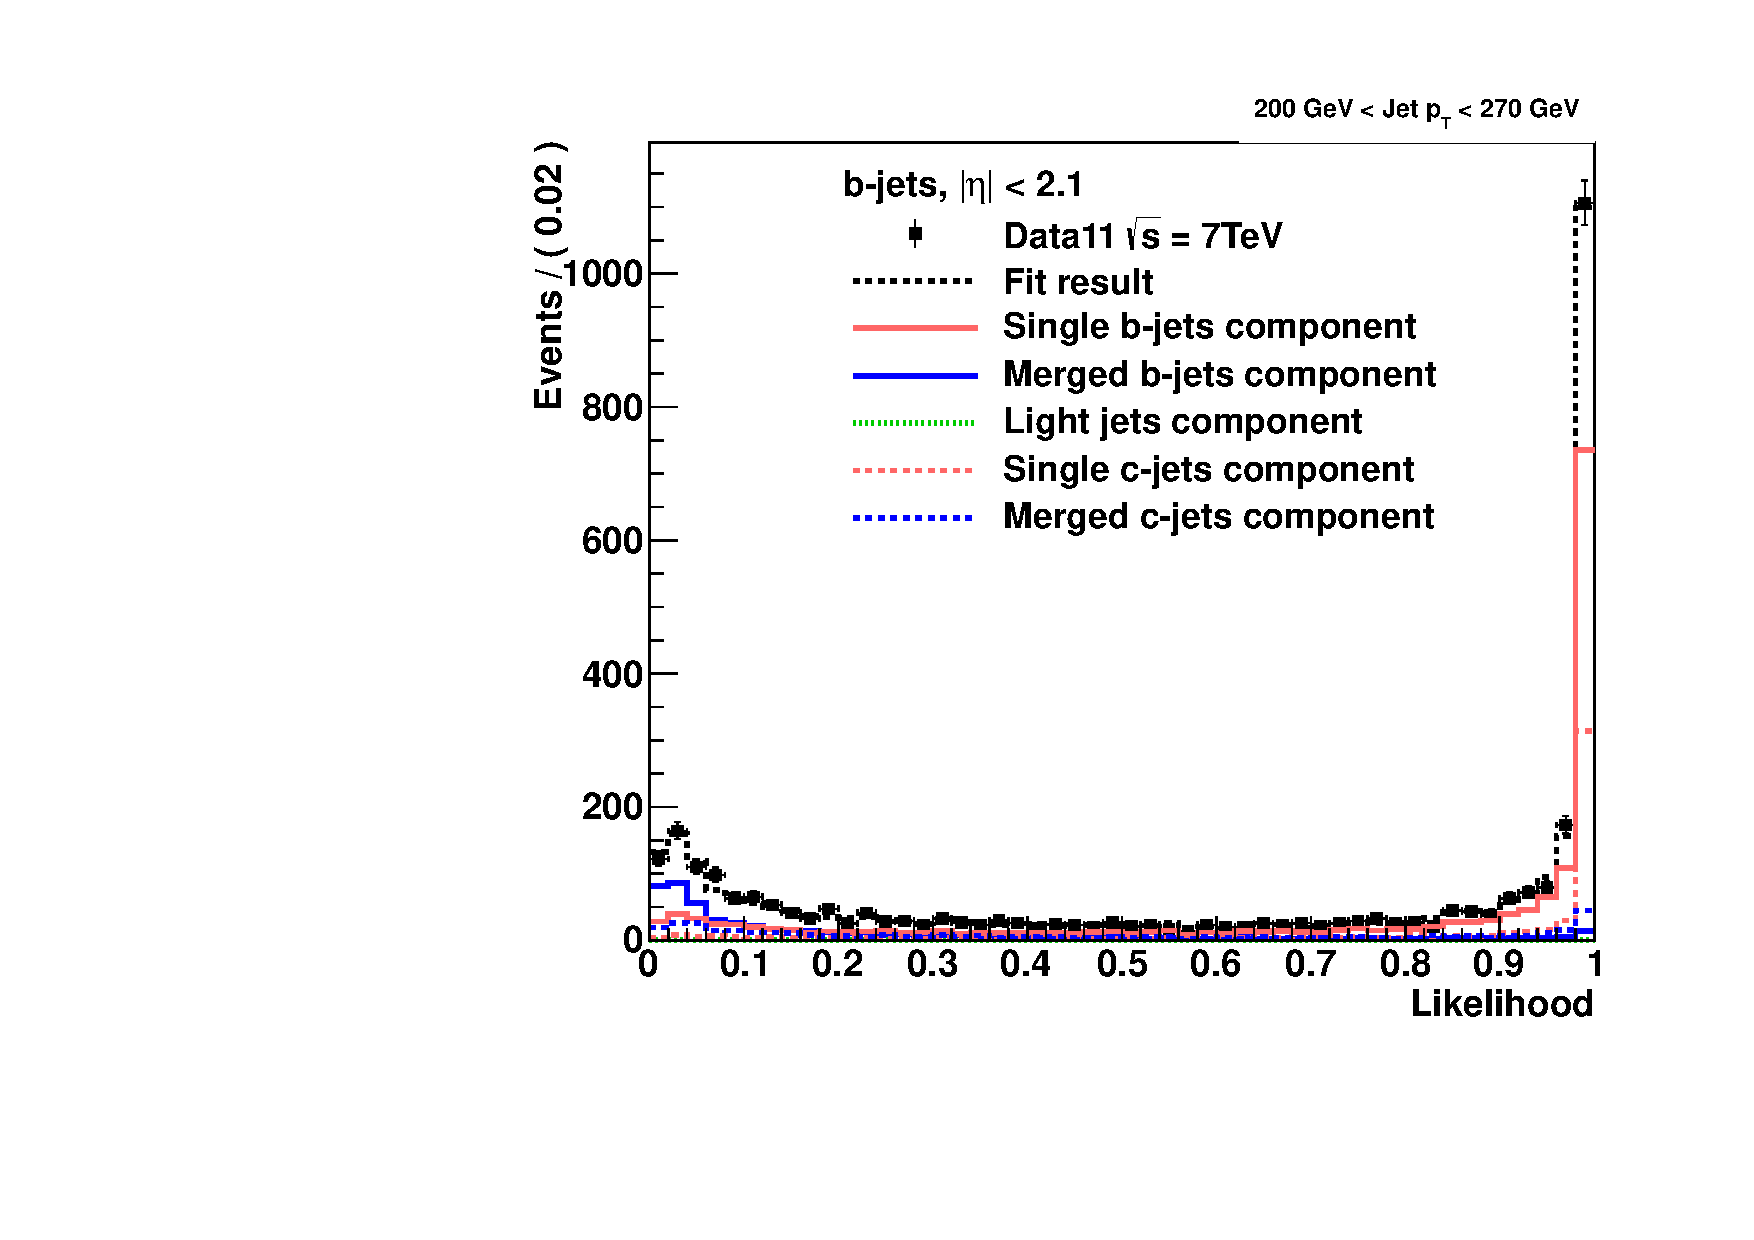
\includegraphics[width=0.7\textwidth]{FIGS/Fits/LikelihoodFit_3param_ETAFull_Bin5.pdf}
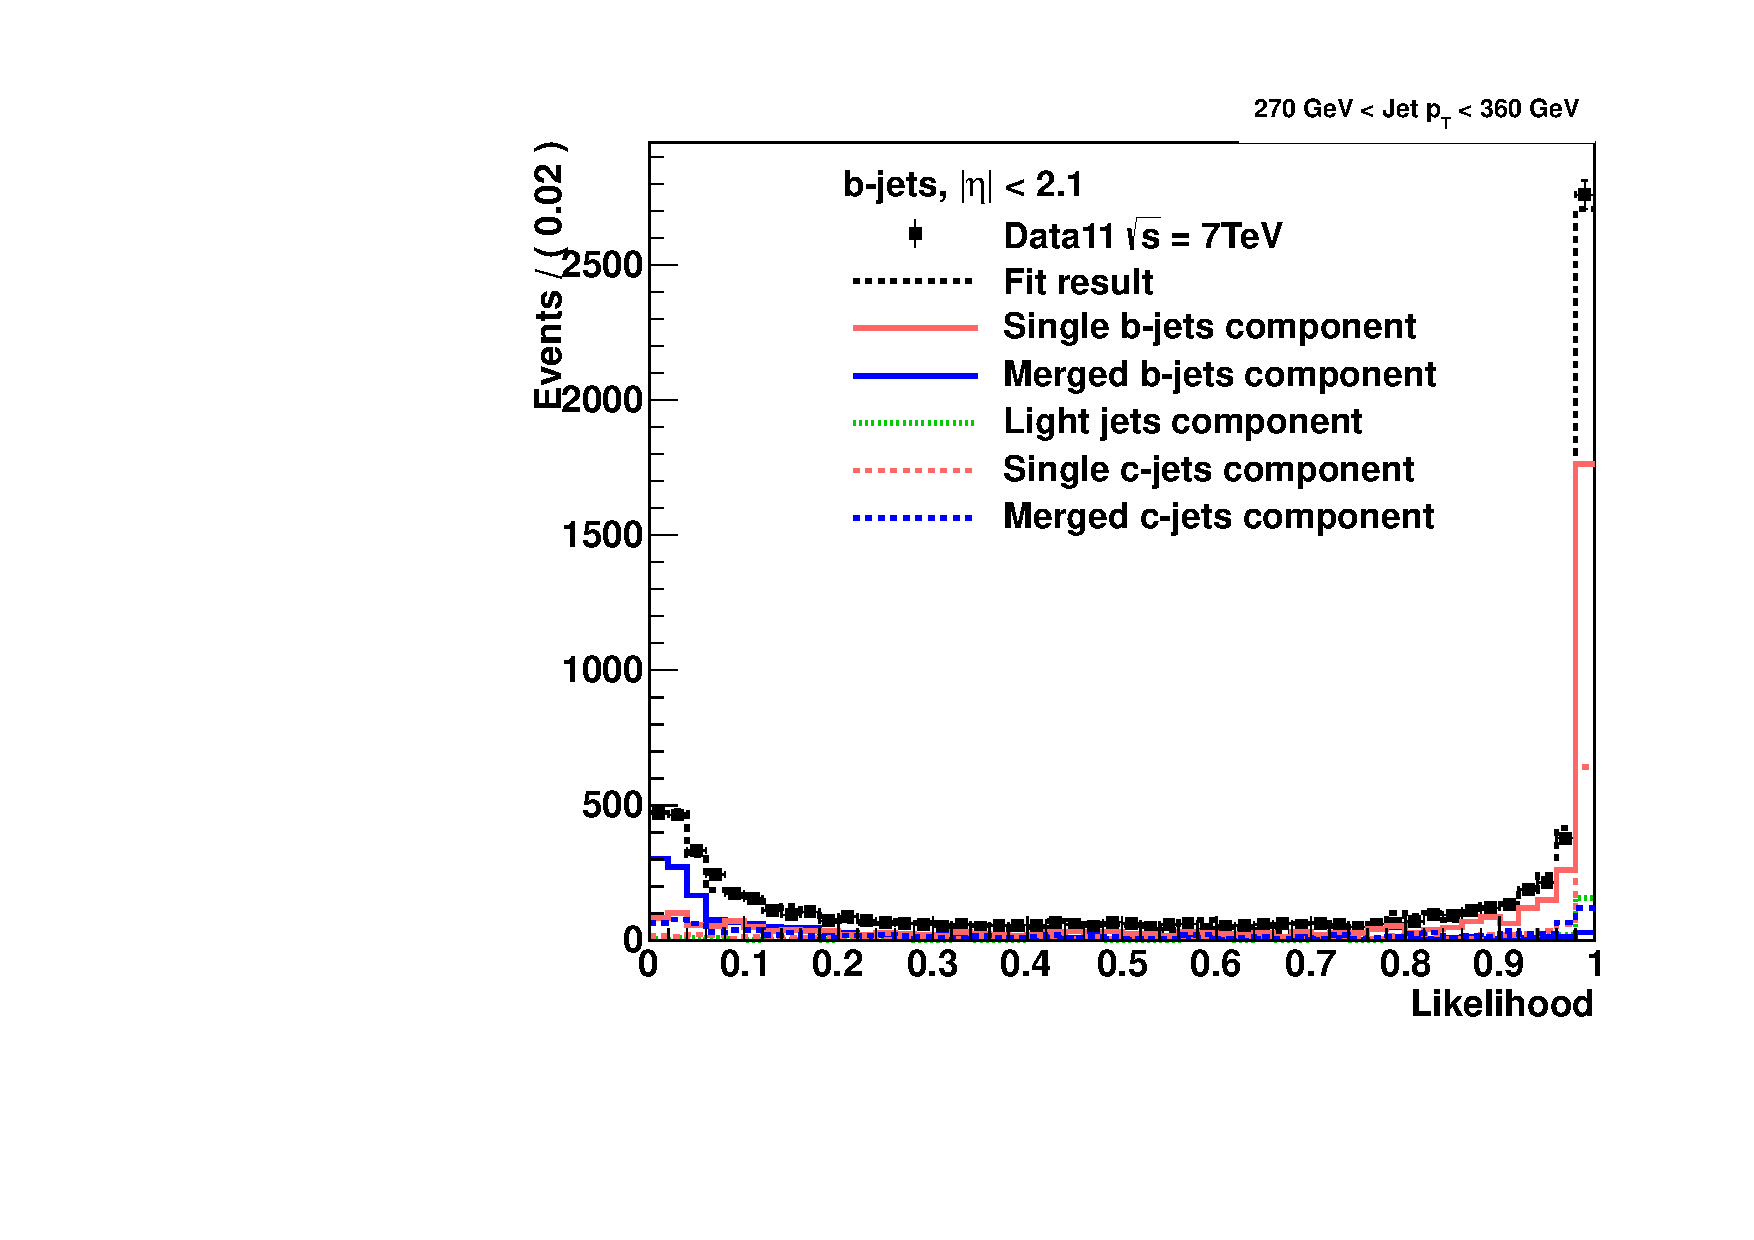
\includegraphics[width=0.7\textwidth]{FIGS/Fits/LikelihoodFit_3param_ETAFull_Bin6.pdf}
\caption{The results of template fits to the likelihood distribution in data. The fits shown here were performed on jets with $\pt$ between  200~GeV and 270~GeV, and 270~GeV and 360~GeV, using five templates of $b$-, $b\bar{b}$-, $c$-, $c\bar{c}$, and light jets.  The ratio of the $c$- to $b$-flavour fractions was fixed to the values observed in the simulation.  Uncertainties shown are for data statistics only.}
\label{fig:fittemplates2}
\end{figure}


%------------------------------------------------------------------------
\section{Systematic uncertainties}\label{sec:FractionSystematics}
%------------------------------------------------------------------------

The systematic uncertainties affecting the method are mainly those that change the shape of the likelihood templates used to fit the sample composition. The following contributions were evaluated:

\begin{itemize}\addtolength{\itemsep}{-0.4\baselineskip}
\item
uncertainty in the track reconstruction efficiency;
\item
uncertainty in the jet transverse momentum resolution 
\item
uncertainty in the jet energy scale.
\item
uncertainty in the heavy flavor fraction
\end{itemize}


In order to calculate the contribution to the total systematic uncertainty from the uncertainty in the track reconstruction efficiency the procedure described in Section~\ref{sec:gbbSystematics} was followed. New likelihood templates were produced and new fits performed. 

The systematic uncertainty originating from the jet  $\pt$ resolution is obtained by smearing the calorimeter jet $\pt$ in the simulation. The likelihood templates were rederived from this ``smeared'' sample, and the likelihood distribution in data was fit using these altered samples. The difference between the unsmeared and the smeared scenarios is taken as a systematic uncertainty. 

The uncertainty originating from the jet energy scale is obtained by scaling the $\pt$ of each jet in the simulation up and down by one standard deviation, according to the uncertainty of the jet energy scale (see Section~\ref{sec:gbbSystematics}), and redoing the likelihood fits on data with the modified $b$, $c$, $b\bar{b}$, $c\bar{c}$ and light templates.

The impact of the uncertainty in the knowledge of the flavour fractions in the simulation was evaluated by increasing the ratio of merged $c$ to merged $b$ fraction in 20\%. This variation only produced a marginal effect on the fit results. The total number of merged $c$ plus merged $b$ did not change showing that, although a separate value for the $b$- and $c$-flavoured components can be obtained, we are,  in reality, measuring the fraction of merged $b+c$ together. The same result is expected if changing the single $c$/single $b$ ratio.

The systematic uncertainties are summarized in Table~\ref{tb:systematicsfits}. The largest ones arise from the jet energy scale and jet transverse momentum resolution.
\begin{table}[!hbt] %[h]
\renewcommand{\arraystretch}{1.2}
\centering
\begin{tabular}{ | c | c |}
\hline
  ~~~~~~~Systematic source~~~~~~~ &~~Uncertainty~~\\ \hline
  track reconstruction efficiency  &    negligible        \\ 
  jet $\pt$ resolution  &    2\%        \\  
  jet energy scale  &    2\%        \\ 
  heavy flavour fraction  &    negligible        \\ \hline 
\end{tabular}
\caption{Systematic uncertainties affecting the template fitting to experimental data.}
\label{tb:systematicsfits}
\end{table}




%------------------------------------------------------------------------
\section{Enriched samples in single and merged $b$-jets}\label{sec:Enriched}
%------------------------------------------------------------------------

The data sample employed in the analysis is $\sim$50\% pured in single $b$-jets, according to the measurements described in Section~\ref{sec:FitsResults}. Having a purer data sample of single or  merged $b$-jets would facilitate the validation of the Monte Carlo templates used for template fitting. To this end we consider the Monte Carlo dijet sample to determine the purity than can be achieved by simple kinematic and $b$-tagging cuts, leaving reasonable statistics.

In a MC parton shower generator such as {\sc Pythia} generator, single $b$-jets are produced mainly via the FCR and FEX processes, while merged $b$-jets are produced 95\% of the time by a gluon splitting into a $b\bar{b}$ pair. In the FCR process two single $b$-quarks are produced in the hard scatter, which lead to two back-to-back $b$-jets. Succesfully tagging these events is a way to construct a sample enriched in single $b$-jets.  On the other hand, events with only one $b$-jet can be produced either in the FEX process, with only one $b$-quark in the final state, or via GSP, where $b\bar{b}$ pairs produced at small angles can be reconstructed as a single $b$-jet. These two scenarios are more difficult to disentangle and will require further selection cuts to be applied.

\subsubsection{Purified sample in single $b$-jets}

To help purifying the sample in single $b$-jets we can then use the $b$-tagging information. Jets in data events with exactly two $b$-tags, selected with MV1 tagging algorithm at its 60\% working point, and satisfying the event and jet selection described in Section~\ref{sec:EventSelection} compose the purified data set.  In order to increase the statistics no requirement on the $\pt$ of the $b$-tagged jets was initially imposed for the event selection. 

Once the enriched sample is obtained, new likelihood fits are performed, for all $\pt$ bin, utilizing the same MC templates as for the nominal data sample in order to evaluate their performance.  
The fractions of single $b$, merged $b$ and light in data recovered, together with their statistical errors and the {\sc Pythia} MC predictions for each $\pt$ bin are displayed in tables~\ref{tb:fitfractions2btagS} to \ref{tb:fitfractions2btagL}.   Examples of these fits are shown  in  Figures~\ref{fig:fitenriched2btag1} and Figures~\ref{fig:fitenriched2btag2}.  The model fitted to the data agrees well within statistics and the result is in agreement with the predictions made by {\sc Pythia} on a sample with the same level of enrichment.  

\subsubsection{Purified sample in merged $b$-jets}

Events with only one $b$-tagged jet were selected for the purification of the data sample in double $b$-hadron jets.  In order to reinforce this selection, a tight anti-b-tagging on any non-tagged jet in the event was implemented.  The anti-b-tagging was performed by imposing, simultaneously, strict cuts on the $b$-tagging weights of the three supported (calibrated) taggers available:
%
\begin{itemize}
\item
MV1:  $w < 0.07$  
\item
JetFitter:  $w < -2$
\item
IP3D+SV1:  $w < -2$
\end{itemize}
%
These weight values correspond to a MV1 tagging efficiency of more than 85\%, and an efficiency for $b$-tagging of more than 80\% for the JetFitter and IP3D+SV1 algorithms. 

The idea behind the anti-b-tagging requirement is to eliminate FCR events for which one of the produced $b$-quark jets failed to be tagged. However, although a certain level of purification was expected, ver little enrichment was achieved with this kind of selection. 

In order to understand this behavior an additional selection was applied: $b$-tagged jets were required to be back-to-back.   %DeltaPhi and DeltaR distributions peak at $\sim \pi$.  
\emph{Most of the $b$-tagged jets are back-to-back. Three topologies are expected to be left after the selection described above: FCR back-to-back single $b$-jets not tagged,  FEX single $b$-jets back-to-back with light jets, and GSP merged $b$-jets, also back-to-back with light.  In 90\% of the cases the second jet is a light jet; consecuently, $b$-jets arising from FEX process constitute the irreducible background for selecting merged $b$-jets. Very little enrichment can be attained.}

 
 







\begin{figure}[tp]
\centering
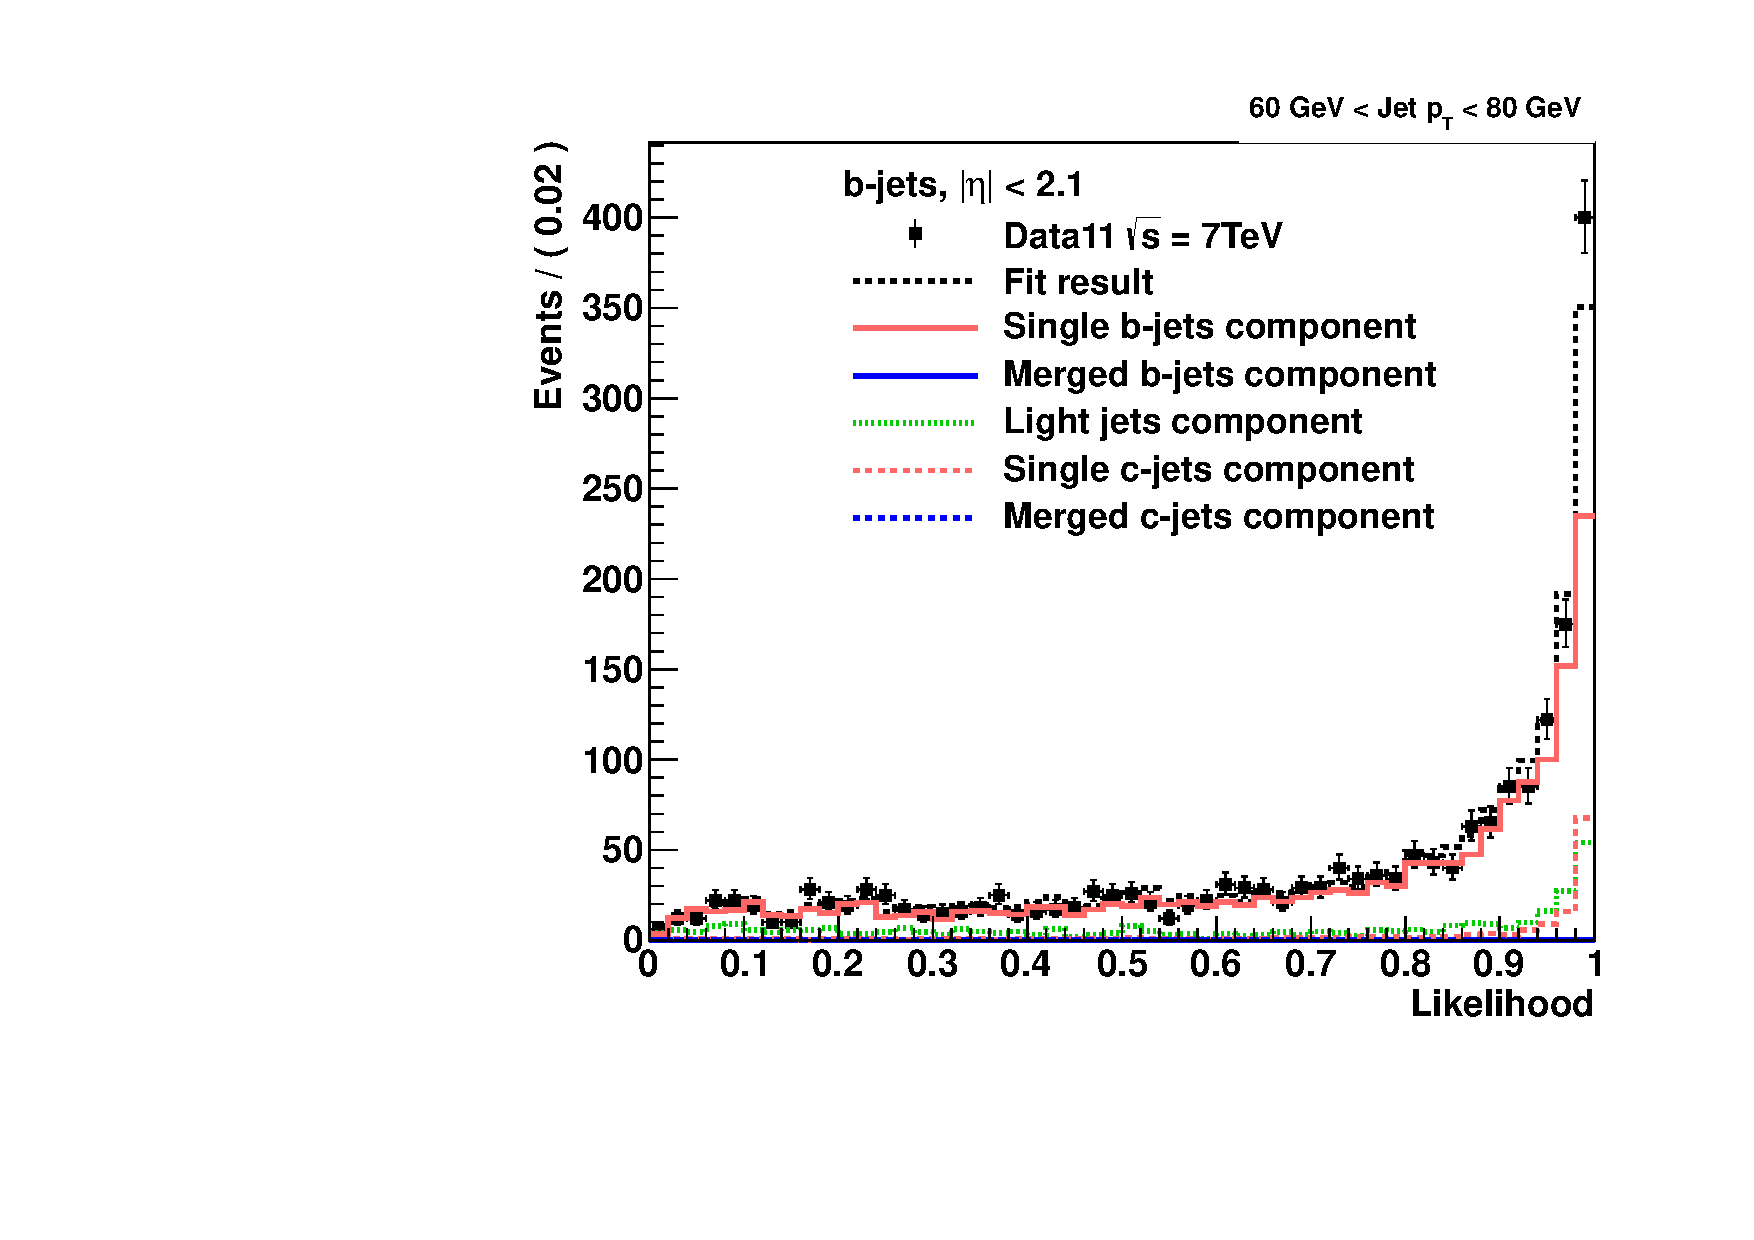
\includegraphics[width=0.7\textwidth]{FIGS/Fits/LikelihoodFit_3param_ETAFull_DataEnriched2btag_Bin1.pdf}
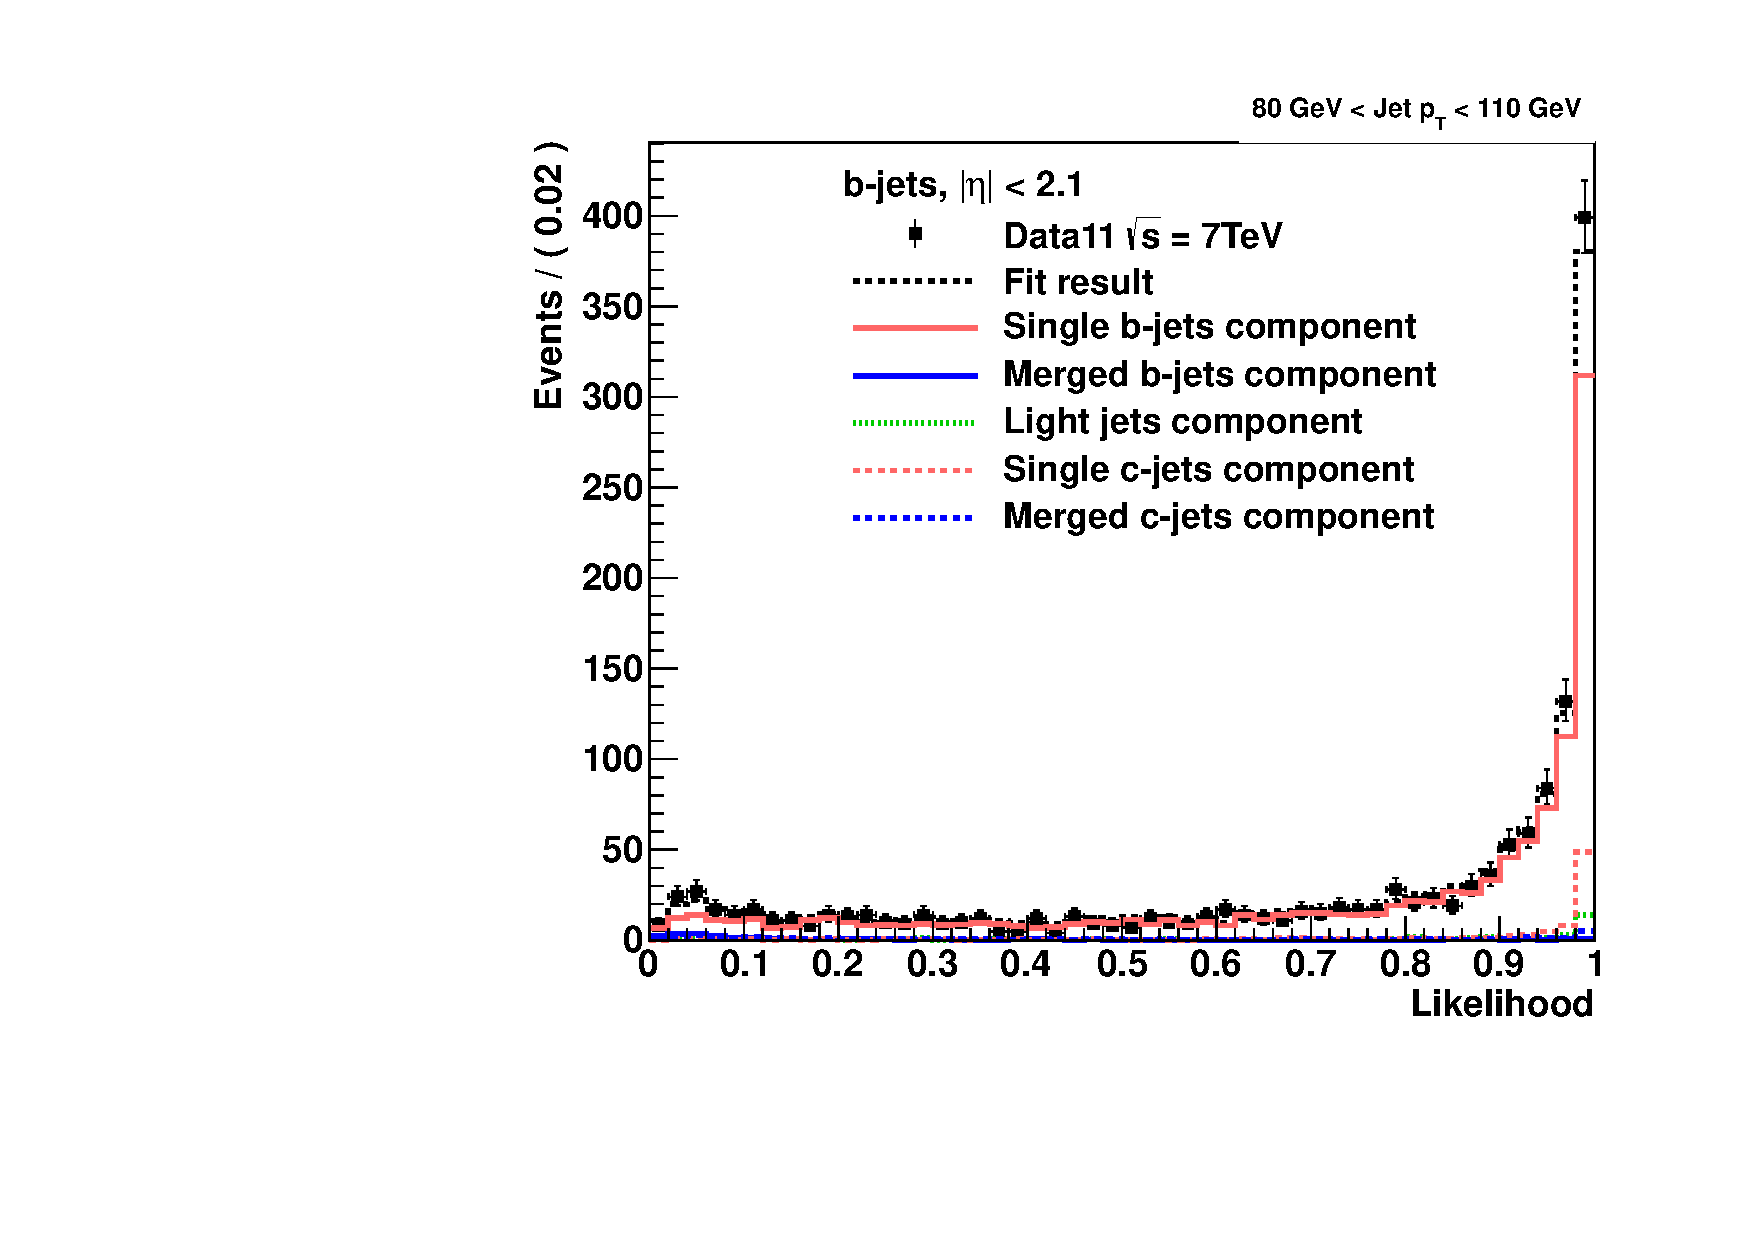
\includegraphics[width=0.7\textwidth]{FIGS/Fits/LikelihoodFit_3param_ETAFull_DataEnriched2btag_Bin2.pdf}
\caption{The results of template fits to the likelihood distribution in data enriched in single $b$-jets. The fits shown here were performed on jets with $\pt$ between  60~GeV and 80~GeV, and 80~GeV and 110~GeV, using five templates of $b$-, $b\bar{b}$-, $c$-, $c\bar{c}$, and light jets.  The ratio of the $c$- to $b$-flavour fractions was fixed to the values observed in the simulation.  Uncertainties shown are for data statistics only.}
\label{fig:fitenriched2btag1}
\end{figure}



\begin{figure}[tp]
\centering
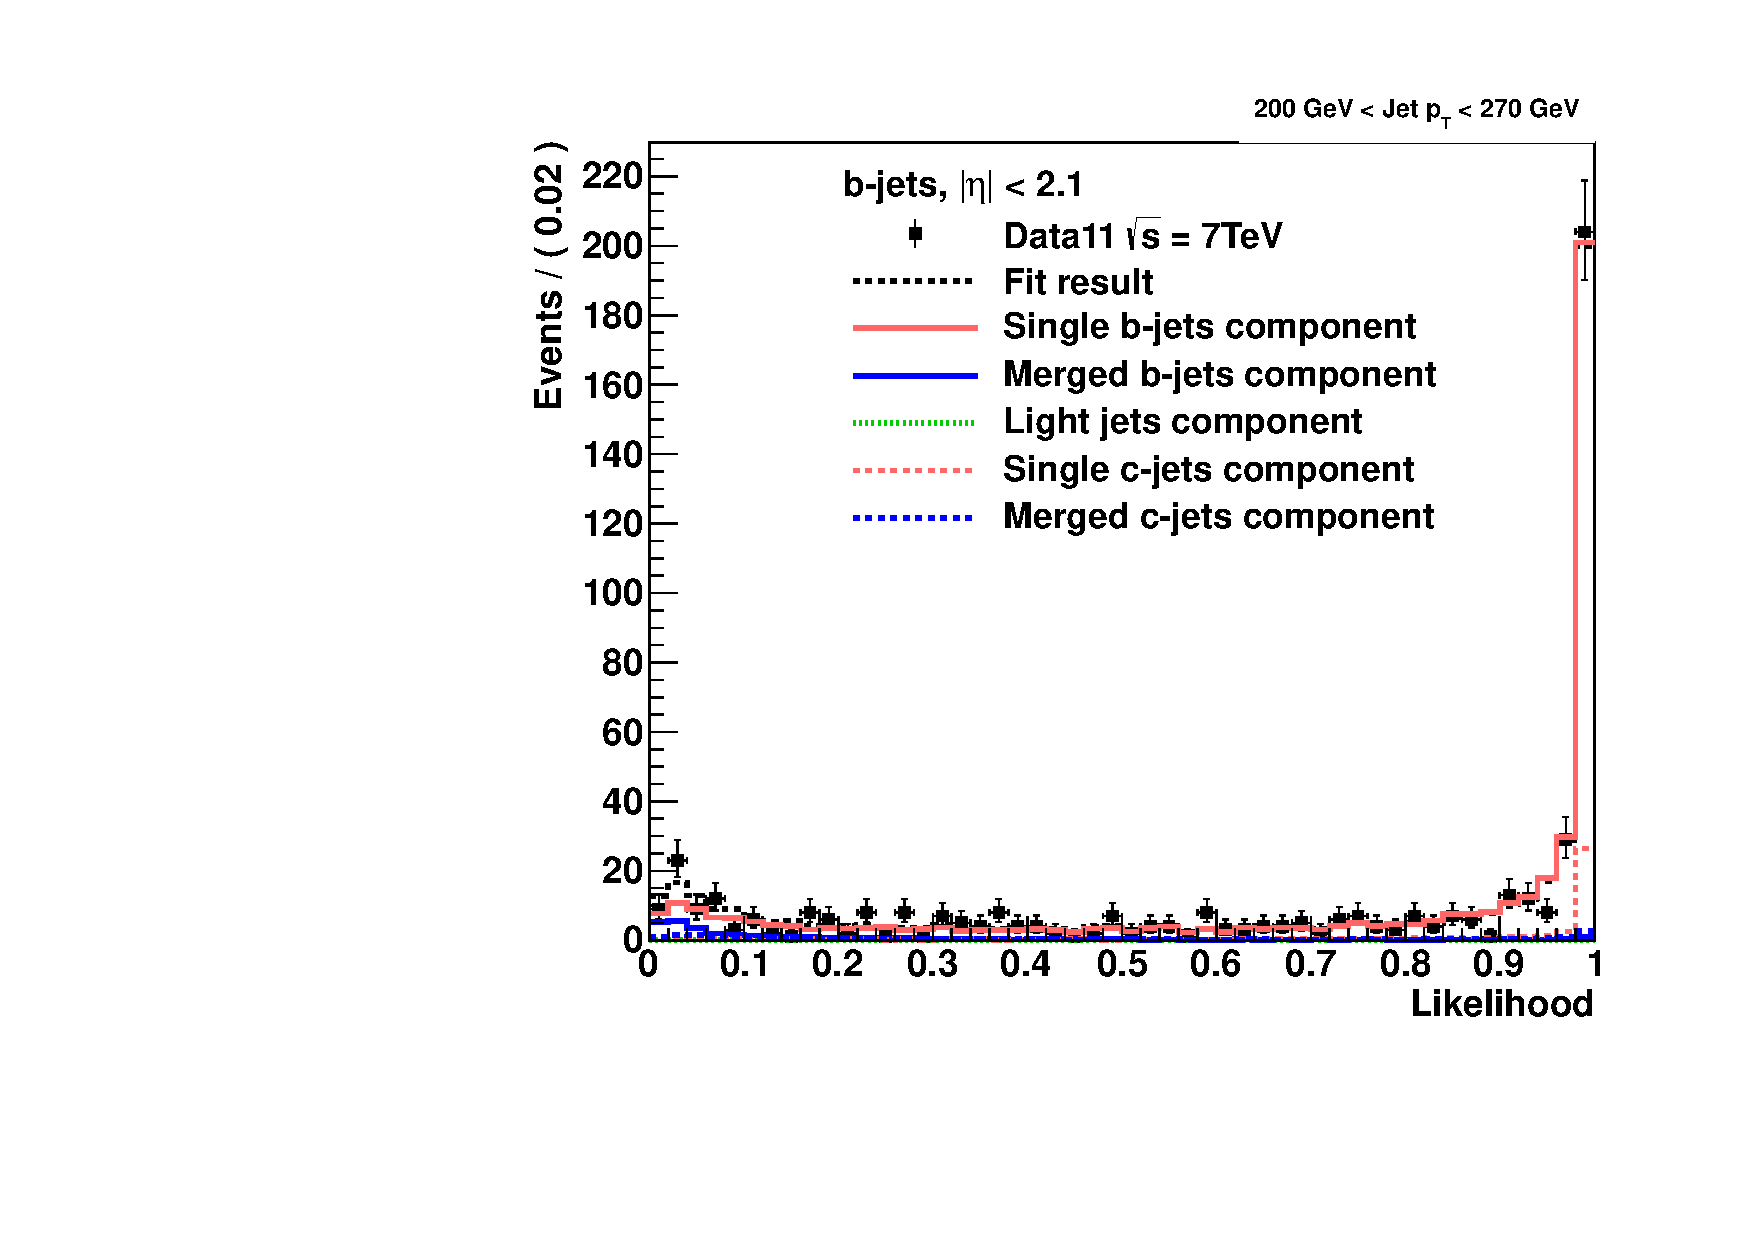
\includegraphics[width=0.7\textwidth]{FIGS/Fits/LikelihoodFit_3param_ETAFull_DataEnriched2btag_Bin5.pdf}
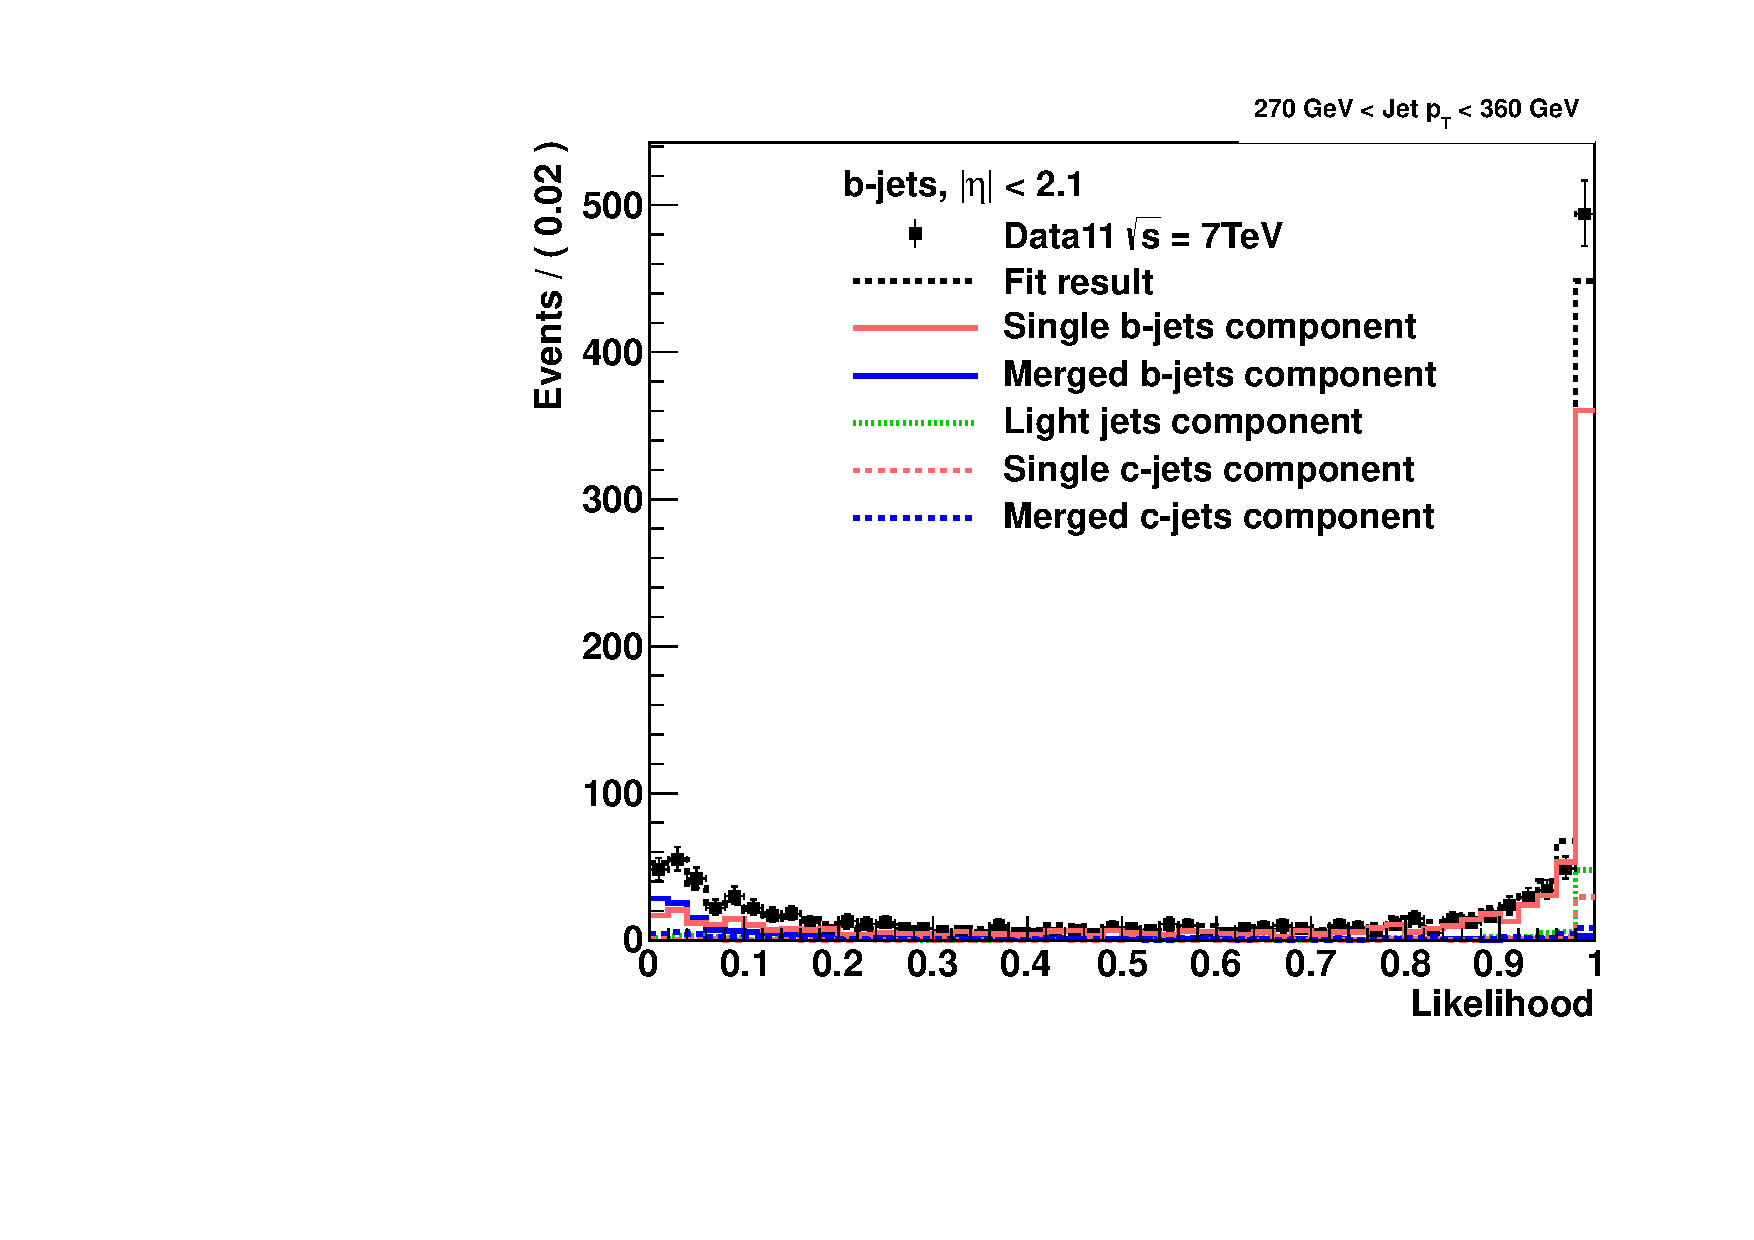
\includegraphics[width=0.7\textwidth]{FIGS/Fits/LikelihoodFit_3param_ETAFull_DataEnriched2btag_Bin6.pdf}
\caption{The results of template fits to the likelihood distribution in data enriched in single $b$-jets. The fits shown here were performed on jets with $\pt$ between  200~GeV and 270~GeV, and 270~GeV and 360~GeV, using five templates of $b$-, $b\bar{b}$-, $c$-, $c\bar{c}$, and light jets.  The ratio of the $c$- to $b$-flavour fractions was fixed to the values observed in the simulation.  Uncertainties shown are for data statistics only.}
\label{fig:fitenriched2btag2}
\end{figure}




\begin{table}[!hbt] %[h]
\renewcommand{\arraystretch}{1.2}
\centering
\begin{tabular}{ | c || c | c | c ||}
  \hline
  Jet $\pt$ & \multicolumn{3}{c||}{single $b$-jet}\\ \cline{2-4}
    (GeV ) & ~~~~fit result~~~ & ~~~~stat.err.~~~~ & pythia prediction \\ \hline
   40 - 60 &  99\%  &  11\%  &  84\% \\  
   60 - 80 &  82\%  &  ~5\%  &  87\% \\ 
   80 - 110&  84\%  &  ~5\%  &  88\% \\ 
  110 - 150&  86\%  &  ~8\%  &  85\% \\ 
  150 - 200&  89\%  &  ~9\%  &  83\% \\ 
  200 - 270&  95\%  &  15\%  &  80\% \\ 
  270 - 360&  67\%  &  11\%  &  81\% \\ 
  360 - 480&  73\%  &  16\%  &  73\% \\ \hline
\end{tabular}
\caption{Measured fractions of single $b$-jets in experimental data from 2011 run, enriched in single $b$-jets.}
\label{tb:fitfractions2btagS}
\end{table}

\begin{table}[!hbt] %[h]
\renewcommand{\arraystretch}{1.2}
\centering
\begin{tabular}{ | c || c | c | c ||}
  \hline
  Jet $\pt$ & \multicolumn{3}{c||}{merged $b$-jet}\\ \cline{2-4}
    (GeV ) & ~~~~fit result~~~ & ~~~~stat.err.~~~~ & pythia prediction \\ \hline
   40 - 60 &  -1\%  &  1\%  &  1\% \\  
   60 - 80 &  -3\%  &  1\%  &  1\% \\ 
   80 - 110&  ~2\%  &  1\%  &  1\% \\ 
  110 - 150&  ~4\%  &  2\%  &  3\% \\ 
  150 - 200&  ~4\%  &  2\%  &  3\% \\ 
  200 - 270&  ~7\%  &  2\%  &  5\% \\ 
  270 - 360&  12\%  &  2\%  &  6\% \\ 
  360 - 480&  10\%  &  1\%  &  8\% \\ \hline
\end{tabular}
\caption{Measured fractions of merged $b$-jets in experimental data from 2011 run, enriched in single $b$-jets.}
\label{tb:fitfractions2btagM}
\end{table}

\begin{table}[!hbt] %[h]
\renewcommand{\arraystretch}{1.2}
\centering
\begin{tabular}{ | c || c | c | c ||}
  \hline
  Jet $\pt$ & \multicolumn{3}{c||}{light $b$-jet}\\ \cline{2-4}
    (GeV ) & ~~~~fit result~~~ & ~~~~stat.err.~~~~ & pythia prediction \\ \hline
   40 - 60 &  ~-7\%  &  11\%  &  5\% \\  
   60 - 80 &  ~17\%  &  ~6\%  &  2\% \\ 
   80 - 110&  ~~4\%  &  ~6\%  &  1\% \\ 
  110 - 150&  ~-1\%  &  ~9\%  &  1\% \\ 
  150 - 200&  ~-6\%  &  10\%  &  2\% \\ 
  200 - 270&  -17\%  &  17\%  &  3\% \\ 
  270 - 360&  ~~9\%  &  11\%  &  4\% \\ 
  360 - 480&  ~~4\%  &  16\%  &  8\% \\ \hline
\end{tabular}
\caption{Measured fractions of light $b$-jets in experimental data from 2011 run, enriched in single $b$-jets.}
\label{tb:fitfractions2btagL}
\end{table}
